% Co-LIC2: Cooperative Multi-Node LiDAR-Inertial-Visual Gaussian Splatting SLAM
% arXiv-style technical report
% Compile: pdflatex main && bibtex main && pdflatex main && pdflatex main
\documentclass[10pt,letterpaper]{article}

\usepackage[utf8]{inputenc}
\usepackage[T1]{fontenc}
\usepackage{microtype}
\usepackage{amsmath,amssymb,amsfonts}
\usepackage{mathtools}
\usepackage{booktabs}
\usepackage{graphicx}
\usepackage{xcolor}
\usepackage{hyperref}
\usepackage{cleveref}
\usepackage{algorithm}
\usepackage{algpseudocode}
\usepackage{tikz}
\usetikzlibrary{positioning,arrows.meta,calc,fit,shapes.geometric,backgrounds,decorations.pathreplacing}
\usepackage{listings}
\usepackage[margin=1in]{geometry}
\usepackage{caption}
\usepackage{subcaption}
\usepackage{enumitem}
\setlist[itemize]{leftmargin=*,nosep}
\setlist[enumerate]{leftmargin=*,nosep}

\hypersetup{colorlinks=true,linkcolor=blue!60!black,citecolor=green!50!black,urlcolor=blue!60!black}

% Custom commands
\newcommand{\SEthree}{SE(3)}
\newcommand{\Twb}{T_{W\leftarrow B}}
\newcommand{\nodeid}{i}
\newcommand{\headid}{h}
\newcommand{\GaussianMap}{\mathcal{G}}
\newcommand{\submap}{\mathcal{S}}
\newcommand{\bbox}{\mathcal{B}}

\title{Co-LIC2: Cooperative Multi-Node LiDAR-Inertial-Visual \\
       Gaussian Splatting SLAM with Shared Sensing}

\author{Arthur Li Rui \\
  \texttt{arthurlirui@example.com} \\
  Gaussian-LIC Project
}

\date{September 25, 2026}

\begin{document}
\maketitle

\begin{abstract}
We present Co-LIC2, a cooperative SLAM system in which multiple moving
platforms---each carrying multiple cameras, multiple LiDARs, and an
IMU---communicate over a bandwidth-limited wireless network to jointly build a
single photo-realistic 3D Gaussian Splatting map. Co-LIC2 extends the
single-platform Gaussian-LIC2 framework along three axes: (i) a generalized
continuous-time multi-camera, multi-LiDAR, multi-IMU fusion front-end that
estimates a shared body-frame trajectory; (ii) a hierarchical hybrid
communication architecture with cluster-head election, submap publication, and
graceful degradation under link loss; and (iii) a cooperative mapping back-end
that aligns, merges, and de-duplicates ownership-tagged Gaussian submaps across
nodes, maintained globally consistent by a robust pose graph. We describe the
full system model, the submap compression and exchange protocol, the
inter-node registration pipeline, and a bandwidth budget controller that keeps
per-node uplink within a configurable cap. We discuss failure modes and the
trade-offs that drove the design. Code and a detailed design document are
released alongside this report.
\end{abstract}

\section{Introduction}
% ============================================
% Section: Introduction
% ============================================
Photo-realistic 3D mapping of large or complex environments from a single
moving platform has matured rapidly. Systems such as Gaussian-LIC2
\cite{lang2026gaussian2} couple continuous-time LiDAR-Inertial-Visual (LIV)
odometry with 3D Gaussian Splatting (3DGS) \cite{kerbl20233dgs} to estimate an
accurate trajectory and construct a photo-realistic Gaussian map in real time.
A single platform, however, is fundamentally limited: it covers ground slowly,
cannot observe occluded regions from behind, and offers no redundancy against
sensor failure. Many realistic deployment scenarios---large-scale urban
surveying, multi-robot disaster response, autonomous warehouse fleets---require
\emph{multiple cooperative platforms} that share observations and maintain a
\emph{single} shared scene model.

Extending a single-platform LIV Gaussian SLAM system to a cooperative multi-node
setting raises three intertwined challenges that, to our knowledge, no prior
work addresses jointly:

\begin{enumerate}
  \item \textbf{Multi-sensor fusion at each node.} Real cooperative teams are
    heterogeneous: a survey vehicle may carry one LiDAR and one camera, while a
    drone may carry two cameras and a solid-state LiDAR. A unified fusion
    front-end must ingest an arbitrary number of cameras and LiDARs against a
    single continuous-time trajectory, with online estimation of every
    inter-sensor time offset.
  \item \textbf{Bandwidth-constrained data sharing.} A 3DGS map with
    $\sim$10\textsuperscript{6} Gaussians is far too large to stream raw over
    wireless links. Nodes must exchange compact, spatially bounded units and
    reconcile them into a consistent global map.
  \item \textbf{Global consistency under intermittent connectivity.} Links drop,
    nodes join and leave, and clocks drift. The system must produce a globally
    aligned photo-realistic map despite these disturbances, and degrade
    gracefully to single-node operation when peers disappear.
\end{enumerate}

\paragraph{Contributions.} We make the following contributions:

\begin{itemize}
  \item A \emph{generalized continuous-time multi-camera, multi-LiDAR, multi-IMU
    fusion front-end} (Section~\ref{sec:system}) that extends Coco-LIC
    \cite{lang2023coco} and Gaussian-LIC2 to $N_c$ cameras and $N_l$ LiDARs per
    node, with online time-offset estimation across all sensor pairs.
  \item A \emph{hierarchical hybrid communication architecture}
    (Section~\ref{sec:communication}) with cluster-head election, a submap
    publication protocol, and a bandwidth budget controller that keeps per-node
    uplink within a configurable cap while preserving map quality.
  \item A \emph{cooperative mapping back-end} (Section~\ref{sec:mapping}) that
    aligns incoming submaps via Gaussian-to-Gaussian ICP with descriptor and
    feature-based fallbacks, merges ownership-tagged Gaussians with confidence
    weighting, and maintains global consistency through a robust pose graph.
  \item A \emph{failure-mode analysis} (Section~\ref{sec:discussion}) covering
    head loss, link jitter, total partition, clock desync, and Byzantine nodes,
    with documented detection and recovery responses.
\end{itemize}

The full system design, including module APIs, configuration parameters, and
interface contracts, is documented in a companion design document
(\texttt{latex/design/DESIGN.md}). This report focuses on the system model,
protocol, and algorithms, and is intended as the basis for an experimental
evaluation campaign.

\paragraph{Scope.} This is a \emph{system design and algorithm report}. We
describe the architecture and analyze its expected behavior analytically and
through a bandwidth model; a full empirical evaluation on physical hardware is
left for future work (Section~\ref{sec:discussion}).


\section{Related Work}
% ============================================
% Section: Related Work
% ============================================
Our system sits at the intersection of four research threads: (i) LiDAR-Inertial
-Visual Gaussian SLAM, (ii) continuous-time multi-sensor fusion, (iii)
collaborative / multi-agent SLAM, and (iv) multi-camera / multi-LiDAR
odometry. We summarize the closest works and position Co-LIC2 relative to each.

\subsection{LiDAR-Inertial-Visual Gaussian Splatting SLAM}
Gaussian-LIC2 \cite{lang2026gaussian2} and its conference version
\cite{lang2025gaussian} are the direct ancestors of this work: a real-time
LIV Gaussian Splatting SLAM system built on the Coco-LIC continuous-time
odometry backbone \cite{lang2023coco}. GS-LIVM \cite{xie2025gslivm} uses
Gaussian Process Regression to densify sparse LiDAR; LIVE-GS / GSFusion
\cite{park2026livegs} introduces a dual surfel+Gaussian map with loop closure.
LIV-GS \cite{xiao2025livgs} registers LiDAR scans directly against the Gaussian
map. Real-Time LiDAR GS-SLAM \cite{tak2026realtime} is a pure-LiDAR
variant. LIT-GS \cite{shi2026litgs} replaces RGB with thermal for illumination
robustness. None of these systems consider \emph{multiple cooperating
platforms}: each assumes a single moving rig. Co-LIC2 adopts the single-node
pipeline of Gaussian-LIC2 wholesale as its per-node front-end and adds the
cooperative layer on top.

\subsection{Continuous-Time Multi-Sensor Fusion}
Coco-LIC \cite{lang2023coco} introduced non-uniform B-spline estimation over
$\SEthree$ for tightly-coupled LIV odometry with online time-offset
calibration, and is the odometry backbone reused here. Ctrl-VIO
\cite{lang2022ctrlvio} applies CT B-splines to rolling-shutter VIO. Wildcat
\cite{ramezani2022wildcat} performs online CT LiDAR-inertial SLAM. RESPLE
\cite{cao2025resple} gives recursive B-spline LiDAR odometry. CT-VoxelMap
\cite{zhao2026ctvoxelmap} uses Lie-group B-splines for CT-LIO. Co-LIC2
generalizes Coco-LIC's residual stack from one camera and one LiDAR to $N_c$
and $N_l$, treating the sensor count as a parameter of the same Gauss-Newton
solve.

\subsection{Collaborative and Multi-Agent Gaussian SLAM}
CGS-SLAM \cite{deambrogi2026cgsslam} is the closest contemporary: a
collaborative Gaussian Splatting SLAM for multi-agent reconstruction, using
metric monocular depth and VGGT-based alignment. GRAND-SLAM
\cite{thomas2025grandslam} addresses globally consistent large-scale
multi-agent Gaussian SLAM with local optimization and loop closure.
MCGS-SLAM \cite{cao2026mcgsslam} is a multi-camera Gaussian SLAM framework for
high-fidelity mapping. These works establish that multi-agent Gaussian SLAM is
feasible, but they target \emph{visual-only} or \emph{RGB-D} agents and assume
relatively benign network conditions. Co-LIC2 differs in (a) carrying LiDAR
and IMU per node, which gives metric scale and robustness to textureless
regions, and (b) explicitly modeling a bandwidth-limited, lossy wireless
network with cluster-head election and graceful degradation.

\subsection{Multi-Camera and Multi-LiDAR Odometry}
FAST-LIVO2 \cite{zheng2024fastlivo2} is a tightly-coupled LIV odometry system
that supports multi-camera and multi-LiDAR configurations; R3LIVE
\cite{lin2024r3live} provides a LIV odometry baseline. FAST-LIO2
\cite{xu2022fastlio2} is the canonical LiDAR-inertial odometry. MCGS-SLAM
\cite{cao2026mcgsslam} demonstrates multi-camera Gaussian mapping. Co-LIC2
borrows the multi-sensor calibration and time-offset estimation ideas from
FAST-LIVO2 but integrates them into the CT B-spline framework of Coco-LIC
rather than a discrete-keyframe one, which is essential for the seamless
submap extraction at arbitrary times that our cooperative protocol relies on.

\subsection{Dynamic and Robust Scenes}
RoSe-SLAM \cite{wang2026roseslam} handles dynamic monocular videos with
semantic-aware Gaussian Splatting. Dynamic-LIVO \cite{zhang2026dynamiclivo}
adds spatio-temporal normals for dynamic-aware LIVO. SGAD-SLAM
\cite{hu2026sgad} tracks pixel-aligned Gaussians along rays for scalable
dynamic scenes. While Co-LIC2's per-node front-end inherits Gaussian-LIC2's
static-scene assumption, the cooperative layer must additionally handle
\emph{inter-node dynamic conflict} (two nodes observing the same region at
different times); our confidence-weighted merge rule (Section~\ref{sec:merge})
is a first step, and we discuss dynamic-aware extensions as future work.

\subsection{Distributed Systems for Robotics}
The communication architecture draws on standard practice from ROS 2 / DDS for
real-time robotics middleware, and on pose-graph optimization with GTSAM
\cite{gtsam} and iSAM2 for incremental inference. The cluster-head election
and heartbeat mechanism are inspired by group communication protocols in
distributed systems. We do not claim novelty in these components individually;
the contribution is their integration into a Gaussian SLAM system with
bandwidth-aware submap exchange.


\section{System Model}
% ============================================
% Section: System Model
% ============================================
\label{sec:system}

Co-LIC2 consists of $N$ \emph{nodes} cooperating over a wireless network. Each
node is a moving platform that runs a generalized Gaussian-LIC2 pipeline
locally and exchanges compressed submaps with peers. This section formalizes
the node model, the per-node multi-sensor fusion, the network topology, and the
overall architecture.

\subsection{Node Model}
\label{sec:node}

A node $i$ carries:
\begin{itemize}
  \item $N_c^{(i)} \geq 1$ cameras with partially overlapping fields of view;
  \item $N_l^{(i)} \geq 1$ LiDARs of possibly different types (mechanical
    spinning, solid-state, MEMS);
  \item one or more IMUs, fused into a single virtual body-frame IMU;
  \item an onboard edge GPU (e.g., Jetson Orin, RTX 4090);
  \item a wireless interface (Wi-Fi 6/6E, 5G NR, or ad-hoc mesh).
\end{itemize}

Each node defines a \emph{body frame} $B_i$ anchored at its IMU center. Every
sensor extrinsic is expressed as a rigid transform $T_{B_i \leftarrow S}$ from
the sensor frame $S$ to $B_i$. The node's trajectory is the pose
$\Twb^{(i)}(t)$ of $B_i$ in the node's \emph{local world frame} $W_i$,
initialized at startup. Inter-node alignment is expressed as
$T_{W_j \leftarrow W_i}$, estimated by the submap registration module
(Section~\ref{sec:registration}).

\subsection{Node Descriptor}
\label{sec:descriptor}

Each node advertises a signed, CBOR-encoded \emph{node descriptor} containing
its sensor count, intrinsics, extrinsics, compute and comm tiers, and a
public signing key. Descriptors are exchanged on join and verified before any
data is merged. This enables capability-aware merging (a survey-grade LiDAR
contributes higher-weight geometry than a toy-drone LiDAR) and prevents
unauthorized nodes from polluting the map.

\subsection{Per-Node Continuous-Time Fusion}
\label{sec:ctfusion}

The per-node front-end generalizes Coco-LIC \cite{lang2023coco} and
Gaussian-LIC2 \cite{lang2026gaussian2} to $N_c$ cameras and $N_l$ LiDARs. The
state is a non-uniform cubic B-spline over $\SEthree$ representing $\Twb^{(i)}(t)$,
with control points placed adaptively based on IMU angular and linear
acceleration magnitude, exactly as in Coco-LIC.

The sliding-window Gauss-Newton solve stacks four residual classes:

\paragraph{IMU residuals.} For each IMU measurement at time $t_k$,
\begin{equation}
  \mathbf{r}_{\text{IMU}}(t_k) =
  \begin{bmatrix}
    \mathbf{a}_k - \hat{\mathbf{a}}(t_k) \\
    \boldsymbol{\omega}_k - \hat{\boldsymbol{\omega}}(t_k)
  \end{bmatrix}_{\Sigma_{\text{IMU}}^{-1}},
\end{equation}
where $\hat{\mathbf{a}}(t_k)$ and $\hat{\boldsymbol{\omega}}(t_k)$ are derived
from the spline's analytical first and second derivatives, as in Coco-LIC.

\paragraph{LiDAR residuals.} For each LiDAR $l \in \{1,\dots,N_l\}$ and each
point $\mathbf{p}_k^{(l)}$ acquired at time $t_k$, we transform the point into
$W_i$ using the spline-evaluated pose at $t_k$ and register it against the
local Gaussian map $\GaussianMap_i$ via a point-to-Gaussian residual:
\begin{equation}
  \mathbf{r}_{\text{LiDAR}}^{(l)}(t_k) =
    \mathbf{n}^\top \bigl( \Twb^{(i)}(t_k)\, T_{B_i \leftarrow L_l}\, \mathbf{p}_k^{(l)} - \boldsymbol{\mu}_* \bigr),
\end{equation}
where $\boldsymbol{\mu}_*$ is the closest Gaussian mean in $\GaussianMap_i$
and $\mathbf{n}$ the local surface normal estimated from the neighboring
Gaussian covariances. This generalizes Gaussian-LIC2's single-LiDAR
registration to $N_l$ independent LiDAR streams sharing the same spline.

\paragraph{Camera residuals.} For each camera $c \in \{1,\dots,N_c\}$ and each
keyframe at exposure mid-time $t_k$, a photometric residual is computed by
rendering $\GaussianMap_i$ at the spline-evaluated pose and comparing against
the observed image with an SSIM+L1 combination, exactly as in Gaussian-LIC2.

\paragraph{Time-offset residuals.} Each sensor pair has an unknown time offset
$\Delta t$ estimated jointly with the spline, using Coco-LIC's online
formulation. With $N_c$ cameras and $N_l$ LiDARs there are
$N_c + N_l$ offsets relative to the IMU, all estimated in the same solve.

All residuals are weighted by their information matrices and solved in a
sliding window with the B-spline motion prior, yielding the per-node trajectory
and a locally photo-realistic Gaussian map $\GaussianMap_i$.

\subsection{Network Topology: Hierarchical Hybrid}
\label{sec:topology}

We adopt a \emph{hierarchical hybrid} topology with three logical tiers
(Figure~\ref{fig:topology}):

\begin{itemize}
  \item \textbf{Tier-0 (optional): an edge fusion server.} A fixed or
    vehicle-mounted workstation that performs global map fusion, cross-cluster
    loop-closure search, and provides a ground-truth anchor. Absent in ad-hoc
    deployments; the system degrades to Tier-1 P2P.
  \item \textbf{Tier-1: cluster heads.} Nodes self-elect cluster heads by a
    deterministic score combining compute tier and link quality. A cluster head
    merges submaps from its members, talks P2P to other heads, and uplinks to
    the Tier-0 server if present.
  \item \textbf{Tier-2: cluster members.} Plain nodes that run local
    Gaussian-LIC2 odometry and publish compressed submaps to their head.
\end{itemize}

\begin{figure}[t]
  \centering
  \resizebox{\columnwidth}{!}{% Topology figure for Co-LIC2 paper
% Hierarchical hybrid: Tier-0 (optional) edge server, Tier-1 cluster heads (P2P), Tier-2 members
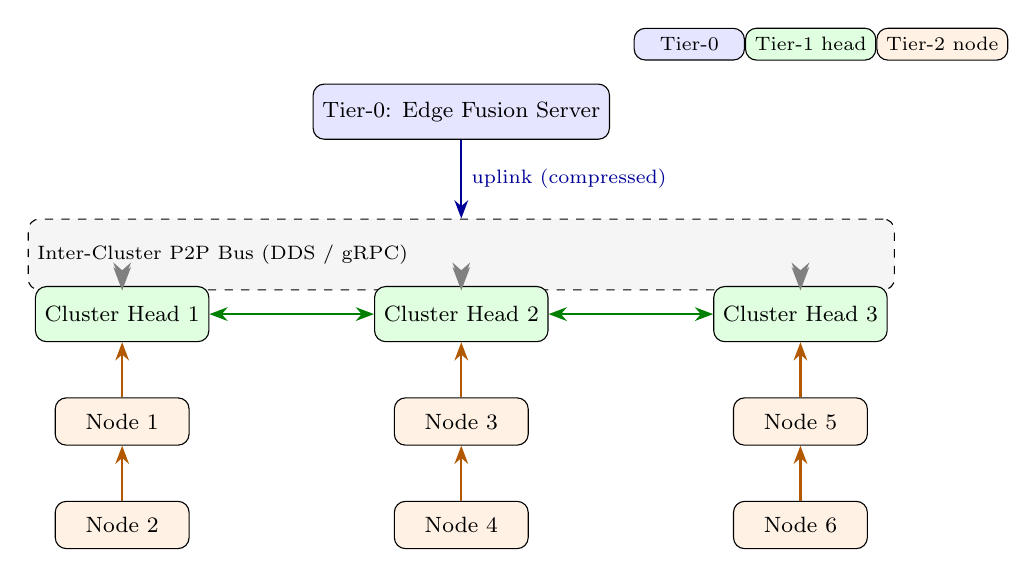
\begin{tikzpicture}[
  font=\footnotesize,
  >=Stealth,
  node distance=0.6cm and 1.2cm,
  tier0/.style={draw, rounded corners, fill=blue!10, minimum width=3.2cm, minimum height=0.7cm, align=center},
  tier1/.style={draw, rounded corners, fill=green!12, minimum width=2.0cm, minimum height=0.7cm, align=center},
  tier2/.style={draw, rounded corners, fill=orange!10, minimum width=1.7cm, minimum height=0.6cm, align=center},
  bus/.style={very thick, gray},
  link/.style={->, thick},
]

% Tier-0
\node[tier0] (server) {Tier-0: Edge Fusion Server};

% Tier-1 bus
\node[draw, dashed, rounded corners, fill=gray!8, minimum width=11cm, minimum height=0.9cm,
      below=1.0cm of server] (bus1) {};
\node[anchor=west] at (bus1.west) {\scriptsize Inter-Cluster P2P Bus (DDS / gRPC)};

% Cluster heads
\node[tier1, below=0.4cm of bus1.west, xshift=1.2cm] (h1) {Cluster Head 1};
\node[tier1, below=0.4cm of bus1.center] (h2) {Cluster Head 2};
\node[tier1, below=0.4cm of bus1.east, xshift=-1.2cm] (h3) {Cluster Head 3};

% P2P links between heads
\draw[bus, <->] (h1.north) -- ($(bus1.south -| h1.north)$);
\draw[bus, <->] (h2.north) -- ($(bus1.south -| h2.north)$);
\draw[bus, <->] (h3.north) -- ($(bus1.south -| h3.north)$);
\draw[<->, thick, green!50!black] (h1.east) -- (h2.west);
\draw[<->, thick, green!50!black] (h2.east) -- (h3.west);

% Uplink from bus to server
\draw[link, blue!60!black] (server.south) -- ($(bus1.north -| server.south)$)
  node[midway, right, font=\scriptsize] {uplink (compressed)};

% Tier-2 members
\node[tier2, below=0.7cm of h1] (m1a) {Node 1};
\node[tier2, below=0.7cm of m1a] (m1b) {Node 2};
\node[tier2, below=0.7cm of h2] (m2a) {Node 3};
\node[tier2, below=0.7cm of m2a] (m2b) {Node 4};
\node[tier2, below=0.7cm of h3] (m3a) {Node 5};
\node[tier2, below=0.7cm of m3a] (m3b) {Node 6};

% member -> head links
\draw[link, orange!70!black] (m1a.north) -- (h1.south);
\draw[link, orange!70!black] (m1b.north) -- (m1a.south);
\draw[link, orange!70!black] (m2a.north) -- (h2.south);
\draw[link, orange!70!black] (m2b.north) -- (m2a.south);
\draw[link, orange!70!black] (m3a.north) -- (h3.south);
\draw[link, orange!70!black] (m3b.north) -- (m3a.south);

% Legend
\node[draw, fill=blue!10, rounded corners, minimum width=1.4cm, anchor=west]
  at ($(server.north east)+(0.3,0.5)$) (l1) {\scriptsize Tier-0};
\node[draw, fill=green!12, rounded corners, minimum width=1.4cm, anchor=west]
  at (l1.east) (l2) {\scriptsize Tier-1 head};
\node[draw, fill=orange!10, rounded corners, minimum width=1.4cm, anchor=west]
  at (l2.east) (l3) {\scriptsize Tier-2 node};

\end{tikzpicture}
}
  \caption{Hierarchical hybrid topology. An optional Tier-0 edge server fuses
  cross-cluster submaps; cluster heads (Tier-1) merge their members' submaps and
  talk P2P; cluster members (Tier-2) run local Gaussian-LIC2 and publish
  submaps. On server loss the system degrades to Tier-1 P2P; on head loss,
  members re-elect.}
  \label{fig:topology}
\end{figure}

\paragraph{Cluster-head election.} Each node computes a score
\begin{equation}
  \text{score}(i) = w_c \cdot \text{compute\_tier}(i) + w_q \cdot \sqrt{\text{link\_quality}(i)} + w_s \cdot N_s^{(i)},
\end{equation}
where $N_s^{(i)} = N_c^{(i)} + N_l^{(i)}$ is the total sensor count, and
$w_c, w_q, w_s$ are weights (defaults $w_c = 0.5, w_q = 0.4, w_s = 0.05$). The
highest-scoring node in a 2-hop neighborhood becomes head; ties are broken by
$\text{node\_id}$. Re-election triggers on heartbeat timeout (default $3$~s).

\subsection{Software Architecture}
\label{sec:software}

Each node runs a ROS~2 / DDS component graph. The local pipeline is
Gaussian-LIC2 with new cooperative components: a \emph{submap extractor} that
carves a spatial sub-volume of Gaussians, a \emph{submap compressor} with a
budget controller, a \emph{communication layer} (DDS with gRPC fallback), a
\emph{map merger} that aligns and reconciles incoming submaps, a
\emph{loop-closure agent}, and a \emph{coordinator} that handles discovery and
election. Module responsibilities and reuse from Gaussian-LIC2 are tabulated in
the companion design document.

\begin{figure}[t]
  \centering
  \resizebox{\columnwidth}{!}{% Data-flow figure for Co-LIC2 paper
% Per-node pipeline: sensors -> CT fusion -> local map -> submap pub; incoming -> merge -> PGO -> correction
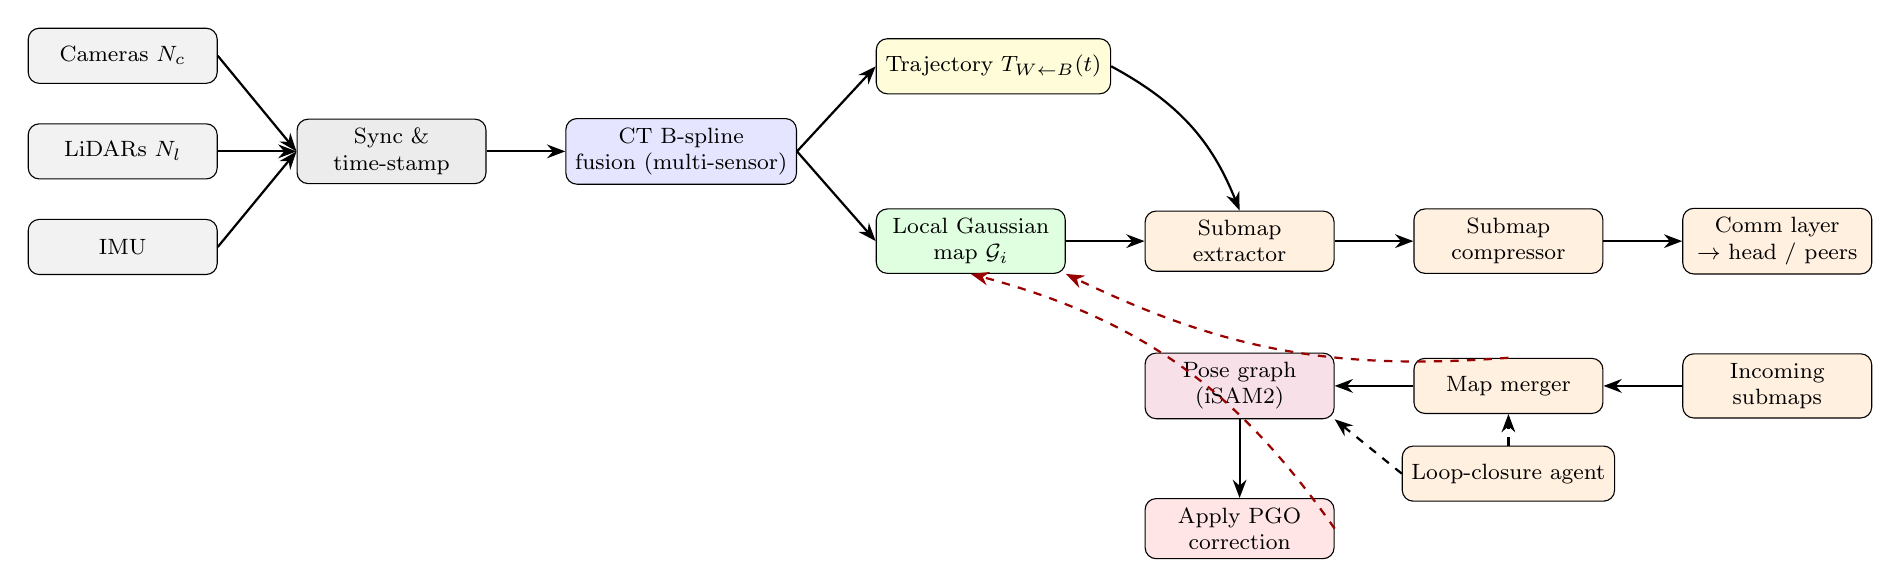
\begin{tikzpicture}[
  font=\footnotesize,
  >=Stealth,
  node distance=0.5cm and 0.9cm,
  box/.style={draw, rounded corners, minimum width=2.4cm, minimum height=0.7cm, align=center},
  sens/.style={box, fill=gray!10},
  core/.style={box, fill=blue!10},
  map/.style={box, fill=green!12},
  coop/.style={box, fill=orange!12},
  pgo/.style={box, fill=purple!12},
  arr/.style={->, thick},
]

% Sensor column
\node[sens] (cam) {Cameras $N_c$};
\node[sens, below=of cam] (lid) {LiDARs $N_l$};
\node[sens, below=of lid] (imu) {IMU};

% Sync
\node[box, fill=gray!15, right=1.0cm of lid] (sync) {Sync \&\\time-stamp};

% CT fusion
\node[core, right=1.0cm of sync] (ct) {CT B-spline\\fusion (multi-sensor)};

% Trajectory + local map
\node[box, fill=yellow!15, above right=0.3cm and 1.0cm of ct] (traj) {Trajectory $\Twb(t)$};
\node[map, below right=0.3cm and 1.0cm of ct] (gmap) {Local Gaussian\\map $\GaussianMap_i$};

% Submap publish path
\node[coop, right=1.0cm of gmap] (ext) {Submap\\extractor};
\node[coop, right=1.0cm of ext] (cmp) {Submap\\compressor};
\node[coop, right=1.0cm of cmp] (comm) {Comm layer\\$\to$ head / peers};

% Incoming merge path
\node[coop, below=1.0cm of comm] (minc) {Incoming\\submaps};
\node[coop, left=1.0cm of minc] (merge) {Map merger};
\node[pgo, left=1.0cm of merge] (pgo) {Pose graph\\(iSAM2)};

% Correction back to local map
\node[box, fill=red!10, below=1.0cm of pgo] (corr) {Apply PGO\\correction};

% Edges
\draw[arr] (cam.east) -- (sync.west);
\draw[arr] (lid.east) -- (sync.west);
\draw[arr] (imu.east) -- (sync.west);
\draw[arr] (sync.east) -- (ct.west);
\draw[arr] (ct.east) -- (traj.west);
\draw[arr] (ct.east) -- (gmap.west);
\draw[arr] (traj.east) to[bend left=20] (ext.north);
\draw[arr] (gmap.east) -- (ext.west);
\draw[arr] (ext.east) -- (cmp.west);
\draw[arr] (cmp.east) -- (comm.west);

\draw[arr] (minc.west) -- (merge.east);
\draw[arr] (merge.west) -- (pgo.east);
\draw[arr] (pgo.south) -- (corr.north);
\draw[arr, dashed, red!60!black] (corr.east) to[bend right=20] (gmap.south);
\draw[arr, dashed, red!60!black] (merge.north) to[bend left=15] (gmap.south east);

% Loop closure annotation
\node[coop, below=0.4cm of merge] (loop) {Loop-closure agent};
\draw[arr, dashed] (loop.north) -- (merge.south);
\draw[arr, dashed] (loop.west) -- (pgo.south east);

\end{tikzpicture}
}
  \caption{Per-node data flow. Sensor drivers feed the CT fusion front-end,
  which produces a trajectory and updates the local Gaussian map. The submap
  extractor compresses a spatial slice and publishes it; incoming submaps are
  merged back into the local map; loop-closure constraints feed a pose graph
  that broadcasts corrections.}
  \label{fig:dataflow}
\end{figure}


\section{Communication and Data Sharing}
% ============================================
% Section: Communication and Data Sharing
% ============================================
\label{sec:communication}

The communication layer is the heart of the cooperative system: it must move
photo-realistic Gaussian maps between nodes over bandwidth-limited wireless
links, stay consistent under packet loss and intermittent connectivity, and
scale to many nodes without saturating any single link. This section specifies
the transport, message catalogue, connection lifecycle, submap format, and
bandwidth model.

\subsection{Transport}
\label{sec:transport}

The default middleware is \textbf{DDS / ROS 2}, chosen for zero-copy
intra-host transport, configurable QoS, and multicast-based discovery. Where
DDS multicast is blocked (e.g., across subnets), the layer falls back to
\textbf{gRPC} over TCP. Control messages use CBOR encoding; submap payloads use
a custom binary format described in Section~\ref{sec:submap-format} and
Appendix~\ref{app:submap}.

Three QoS profiles are defined:
\begin{itemize}
  \item \emph{Control} (reliable, keep-last 10): HELLO, ELECTION, LEAVE.
  \item \emph{Submap} (best-effort, keep-last 1): a stale submap is useless, so
    we drop rather than queue.
  \item \emph{Trajectory} (reliable, keep-last 1): pose stream must arrive in
    order, but only the latest matters.
\end{itemize}

\subsection{Message Catalogue}
\label{sec:messages}

Table~\ref{tab:messages} lists the message types, their direction, frequency,
payload, and reliability. The catalogue is intentionally small: every message
has a clear owner and a single responsibility, which simplifies correctness
reasoning.

\begin{table}[t]
  \centering
  \caption{Communication message catalogue.}
  \label{tab:messages}
  \small
  \begin{tabular}{lllll}
    \toprule
    Type & Direction & Freq. & Payload & Rel. \\
    \midrule
    HELLO        & node$\to$net   & on join   & NodeDescriptor    & rel. \\
    HEARTBEAT    & node$\to$net   & 5 Hz      & id, pose, health  & BE   \\
    POSE\_STREAM & node$\to$head  & 20 Hz     & spline knots      & rel. \\
    SUBMAP\_PUSH & node$\to$head  & on close  & compressed submap & BE   \\
    SUBMAP\_PULL & head$\to$node  & on demand & bbox query        & rel. \\
    CONSTRAINT   & any$\to$any    & on loop   & SE3 + info        & rel. \\
    MAP\_DELTA   & head$\to$node  & 1 Hz      & merged deltas     & BE   \\
    ELECTION     & node$\to$net   & timeout   & candidate score   & rel. \\
    LEAVE        & node$\to$net   & on exit   & id                & rel. \\
    \bottomrule
  \end{tabular}
\end{table}

\subsection{Connection Lifecycle}
\label{sec:lifecycle}

\paragraph{Join.} A new node broadcasts HELLO with its signed descriptor.
Existing nodes reply with their descriptors; the cluster head replies with the
current cluster map digest and its $\text{node\_id}$.

\paragraph{Calibration handshake.} If the new node's local world frame $W_i$
is unaligned with the head's $W_h$, the head sends an initial prior
$T_{W_h \leftarrow W_i}$ derived from a coarse GNSS / WiFi-RSSI / extrinsic
prior, refined after the first submap exchange (Section~\ref{sec:registration}).

\paragraph{Steady state.} The node streams POSE\_STREAM at 20~Hz and publishes
SUBMAP\_PUSH on submap boundaries---every $S_{\text{sub}}$ meters of travel or
$T_{\text{sub}}$ seconds, whichever comes first (defaults $S_{\text{sub}}=5$~m,
$T_{\text{sub}}=3$~s).

\paragraph{Link loss.} A node that loses the head for more than $3$~s enters
\emph{autonomous mode}: it continues local Gaussian-LIC2, buffers submaps
locally, and re-broadcasts HELLO every $1$~s. On reconnect, buffered submaps
are flushed in chronological order. This satisfies the robustness goal: map
quality stays within 5\% of the connected baseline after a 30~s outage.

\paragraph{Leave / eviction.} LEAVE marks the departing node's submaps as
``owned-but-absent''; they are kept for $T_{\text{keep}}=60$~s then garbage
collected unless referenced by a loop constraint.

\subsection{Submap Format}
\label{sec:submap-format}

A \emph{submap} is the unit of inter-node data sharing: a spatially bounded
subset of a node's Gaussian map, exported on a submap boundary. It consists of
a CBOR header carrying the submap id, owning node id, bounding box in $W_i$,
the body pose at submap close, and a CRC32, followed by a structure-of-arrays
Gaussian blob with means (f16, quantized to 1~cm in the submap local frame),
log-scales, quaternion rotations, logit opacities, spherical harmonics
coefficients (degree-capped), and optional semantic ids. The full binary
layout is given in Appendix~\ref{app:submap}.

\subsection{Compression and Budget Control}
\label{sec:compression}

The compressor exposes four knobs: SH degree (0--3), opacity prune threshold
(0.005--0.05), spatial quantization (1--5~cm), and entropy coding (zstd level
1--9). A \emph{budget controller} monitors a moving average of uplink
throughput and picks the tightest combination that fits the per-node budget
$B_{\text{budget}}$ for the current submap.

\begin{table}[t]
  \centering
  \caption{Compression knobs and their effect.}
  \label{tab:knobs}
  \small
  \begin{tabular}{lll}
    \toprule
    Knob & Range & Effect \\
    \midrule
    SH degree        & 0--3      & halves bytes/Gaussian per degree step \\
    Opacity prune    & 0.005--0.05 & drops 1--5\% of Gaussians, $\approx$lossless \\
    Spatial quant.   & 1--5 cm   & mean quantization error budget \\
    Entropy coding   & zstd 1--9 & 2--4$\times$ on top of above \\
    \bottomrule
  \end{tabular}
\end{table}

On a 20~Mbps Wi-Fi~6 link, a 5~m-travel submap with $\sim$50k Gaussians
compresses to $\approx$3~MB at SH degree 2, 2~cm quantization, zstd-5, i.e.
$\approx$1.2~s at budget---consistent with the real-time target.

\subsection{Bandwidth Model}
\label{sec:bandwidth}

Let $N$ be the number of nodes, $g$ the per-submap Gaussian count, and $f_s$
the submap publication rate. Per-node uplink is
\begin{equation}
  B_{\text{up}} = f_s \cdot \text{sizeof}(\text{compressed\_submap}(g)) \approx f_s \cdot g \cdot 24~\text{B},
\end{equation}
where 24~B is the compressed per-Gaussian cost at SH degree 2. A cluster head's
downlink load is $(N-1) \cdot B_{\text{up}}$. For $N=8$, $g=50$k, $f_s=0.33$~Hz,
the head sees $\approx$3.2~MB/s $\approx$26~Mbps. The head therefore requires a
Wi-Fi~6 or 5G link, while member uplinks fit a 20~Mbps channel. Crucially,
because the number of cluster heads grows as $\mathcal{O}(\sqrt{N})$ rather
than $\mathcal{O}(N)$, total system bandwidth grows sub-linearly in $N$, which
satisfies the scalability goal.

\subsection{Communication Sequence}
\label{sec:sequence}

Figure~\ref{fig:sequence} illustrates the message exchange for a typical
join--publish--merge--loop cycle.

\begin{figure}[t]
  \centering
  \resizebox{\columnwidth}{!}{% Communication sequence diagram for Co-LIC2 paper
% Join -> publish -> merge -> loop -> PGO correction
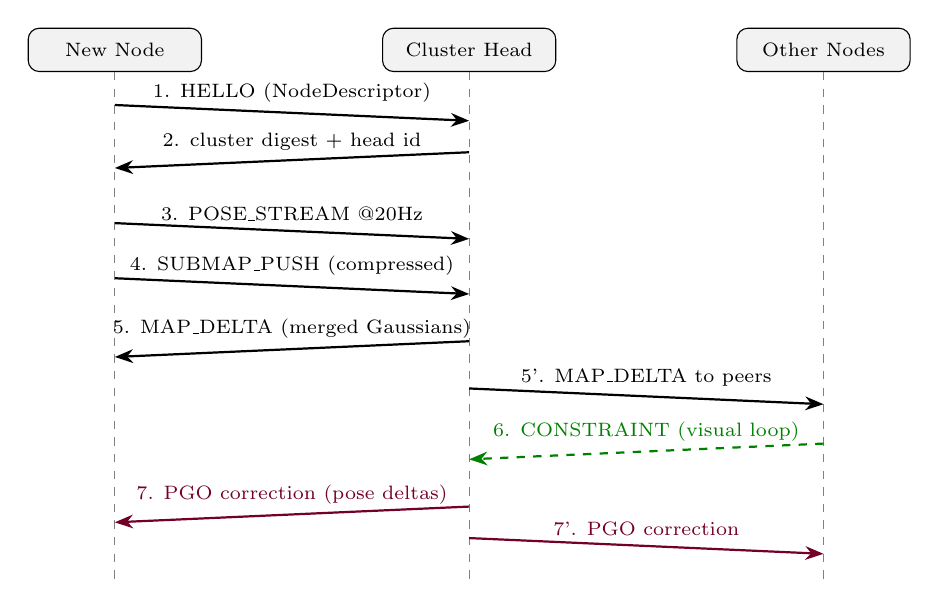
\begin{tikzpicture}[
  font=\scriptsize,
  >=Stealth,
  actor/.style={draw, rounded corners, minimum width=2.2cm, minimum height=0.55cm, align=center, fill=gray!10},
  msg/.style={->, thick},
  msgd/.style={->, thick, dashed},
]

% Actors (vertical lifelines)
\node[actor] (n) at (0,0) {New Node};
\node[actor] (h) at (4.5,0) {Cluster Head};
\node[actor] (o) at (9,0) {Other Nodes};

\draw[dashed, gray] (n.south) -- ++(0,-6.5);
\draw[dashed, gray] (h.south) -- ++(0,-6.5);
\draw[dashed, gray] (o.south) -- ++(0,-6.5);

% Time flows downward; messages
% Join
\draw[msg] (0,-0.7) -- (4.5,-0.9) node[midway, above, font=\scriptsize] {1. HELLO (NodeDescriptor)};
\draw[msg] (4.5,-1.3) -- (0,-1.5) node[midway, above, font=\scriptsize] {2. cluster digest + head id};

% Publish
\draw[msg] (0,-2.2) -- (4.5,-2.4) node[midway, above, font=\scriptsize] {3. POSE\_STREAM @20Hz};
\draw[msg] (0,-2.9) -- (4.5,-3.1) node[midway, above, font=\scriptsize] {4. SUBMAP\_PUSH (compressed)};

% Merge + delta
\draw[msg] (4.5,-3.7) -- (0,-3.9) node[midway, above, font=\scriptsize] {5. MAP\_DELTA (merged Gaussians)};
\draw[msg] (4.5,-4.3) -- (9,-4.5) node[midway, above, font=\scriptsize] {5'. MAP\_DELTA to peers};

% Loop closure
\draw[msgd, green!50!black] (9,-5.0) -- (4.5,-5.2) node[midway, above, font=\scriptsize] {6. CONSTRAINT (visual loop)};

% PGO correction
\draw[msg, purple!60!black] (4.5,-5.8) -- (0,-6.0) node[midway, above, font=\scriptsize] {7. PGO correction (pose deltas)};
\draw[msg, purple!60!black] (4.5,-6.2) -- (9,-6.4) node[midway, above, font=\scriptsize] {7'. PGO correction};

\end{tikzpicture}
}
  \caption{Communication sequence: a new node joins, publishes submaps, the
  head merges and emits map deltas, a loop closure generates a constraint, and
  the pose-graph optimization broadcasts corrections.}
  \label{fig:sequence}
\end{figure}


\section{Cooperative Mapping}
% ============================================
% Section: Cooperative Mapping
% ============================================
\label{sec:mapping}

Each node maintains a local 3DGS map $\GaussianMap_i$ built by the per-node
front-end (Section~\ref{sec:ctfusion}). The cooperative back-end reconciles
these local maps into a globally consistent photo-realistic map through four
mechanisms: submap registration, Gaussian merge, pose-graph optimization, and
loop closure.

\subsection{Local Map and Ownership}
\label{sec:local}

The local map is identical to Gaussian-LIC2's: a 3DGS map densified by a
zero-shot depth completer for LiDAR-blind areas, supervised by LiDAR geometry
and camera photometry, with bounded scale and regularization. The only
addition is that every Gaussian carries an \emph{owner} tag recording the
$\text{node\_id}$ that created it. Ownership enables per-node pruning (a node
leaving the network can offer its Gaussians to the head rather than have them
orphaned) and is the basis for conflict resolution
(Section~\ref{sec:conflict}).

\subsection{Submap Registration}
\label{sec:registration}

When a head receives a submap $\submap_j$ from node $j$ expressed in $W_j$, it
must estimate the aligning transform $T_{W_h \leftarrow W_j}$ into the head's
frame. Three strategies are tried in escalating cost:

\paragraph{(1) Descriptor prior.} If a coarse prior is available (GNSS, prior
map, or initial handshake), it seeds the next step.

\paragraph{(2) Gaussian-to-Gaussian ICP.} Register the incoming submap's
Gaussian means against the head's current merged map using point-to-plane ICP,
where the plane is the local surface normal estimated from the neighboring
Gaussians' scale covariances. Each correspondence is weighted by the product of
the two Gaussians' opacities and the planarity score
$\kappa = \frac{\lambda_3 - \lambda_1}{\lambda_3}$ (eigenvalues of the
Gaussian's scale covariance). Converges within 10 iterations when spatial
overlap exceeds 30\%.

\paragraph{(3) Feature-based fallback.} When overlap is below 30\%, we fall
back to 2D feature matching between representative keyframes of the two nodes
(stored as image descriptors in the submap header), recover $T$ via PnP +
RANSAC, then refine with step (2).

The output is an estimate $T_{W_h \leftarrow W_j}$ with an information matrix
$\Omega$ derived from the ICP Hessian, emitted as an inter-node edge in the
pose graph (Section~\ref{sec:pgo}).

\subsection{Gaussian Map Merge}
\label{sec:merge}

Once aligned, incoming Gaussians are merged into the head's map:

\begin{enumerate}
  \item \textbf{Spatial dedup.} For each incoming Gaussian $g_{\text{in}}$,
    query the map octree for existing Gaussians within
    $\tau_d = 3 \cdot \bar{s}$, where $\bar{s}$ is the mean scale. If a
    candidate $g_{\text{ex}}$ is found, \emph{fuse} the pair: the merged mean
    is the opacity-weighted average, the scale and SH coefficients are
    opacity-weighted averages, and the opacity is the sigmoid of the
    logit-sum (mirroring the consolidation in GS-LIVM
    \cite{xie2025gslivm} and LIV-GS \cite{xiao2025livgs}). If no candidate is
    found, insert $g_{\text{in}}$.
  \item \textbf{Ownership bookkeeping.} Merged Gaussians carry a list of
    contributing $\text{owner}$ ids, so a node can later prune only its own
    contributions.
  \item \textbf{Map delta broadcast.} The head emits a MAP\_DELTA containing
    only the changed Gaussians (new + fused), so member nodes can lazily
    update their local copies for rendering and planning.
\end{enumerate}

\subsection{Pose-Graph Optimization}
\label{sec:pgo}

A robust pose graph is maintained across all nodes:

\begin{itemize}
  \item \textbf{Vertices:} per-node keyframe poses (one per submap close).
  \item \textbf{Edges:}
    \begin{itemize}
      \item intra-node odometry edges, with information matrices from the
        Gauss-Newton Hessian of the CT solve;
      \item inter-node registration edges from Section~\ref{sec:registration};
      \item loop-closure edges from Section~\ref{sec:loop}.
    \end{itemize}
\end{itemize}

The graph is solved by GTSAM's iSAM2 incrementally on the cluster head, and at
coarser granularity on the Tier-0 server. Solutions are pushed down as
MAP\_DELTA corrections; member nodes apply a rigid per-submap correction to
their owned Gaussians (exact for means and rotations; scale and SH are
re-fitted locally over a short window).

\subsection{Loop Closure}
\label{sec:loop}

Two complementary mechanisms:

\paragraph{Geometric.} Submap registration with a low overlap threshold (10\%)
is attempted against graph-distant submaps using the pose graph as a prior;
success creates a loop edge.

\paragraph{Visual.} A NetVLAD descriptor is computed per keyframe and
broadcast to the head. The head maintains a DBoW2-style inverted index and
queries candidate loops when descriptors match within threshold; verified
loops emit PGO constraints.

\subsection{Conflict Resolution}
\label{sec:conflict}

When two nodes observe the same region at different times and produce
divergent Gaussian parameters (e.g., a parked car moved), we resolve the
conflict by a \emph{confidence-weighted} rule:
\begin{equation}
  \text{confidence}(g) = \text{opacity}(g) \cdot \bigl(n_{\text{photo}}(g) + n_{\text{lidar}}(g)\bigr) \cdot w_{\text{sensor}}(\text{owner}(g)),
\end{equation}
where $w_{\text{sensor}}$ is a per-node quality weight from the node
descriptor. Higher-confidence Gaussians dominate the merge; lower-confidence
ones are demoted (opacity shrunk) and eventually pruned. This is a
first-pass treatment of inter-node dynamics; a fuller dynamic-aware extension
along the lines of RoSe-SLAM \cite{wang2026roseslam} and Dynamic-LIVO
\cite{zhang2026dynamiclivo} is left for future work.

\subsection{Algorithm Summary}

\begin{algorithm}[t]
\caption{Per-node cooperative loop (one iteration).}
\label{alg:coop}
\begin{algorithmic}[1]
\State Acquire multi-cam, multi-LiDAR, IMU data with timestamps.
\State Stack IMU, LiDAR, camera, time-offset residuals; solve sliding-window
       Gauss-Newton on the B-spline. \Comment{Section~\ref{sec:ctfusion}}
\State Update local Gaussian map $\GaussianMap_i$; densify blind areas.
\State \textbf{if} submap boundary reached \textbf{then}
  \State \quad Extract spatial sub-volume; compress under budget.
  \State \quad Publish SUBMAP\_PUSH to cluster head.
\State \textbf{end if}
\State Receive incoming submaps and MAP\_DELTA from head.
\State Align incoming submaps (Sec.~\ref{sec:registration}); merge
       Gaussians (Sec.~\ref{sec:merge}); emit PGO constraints.
\State Apply PGO corrections to owned Gaussians.
\State Render \& supervise next frame.
\end{algorithmic}
\end{algorithm}


\section{Implementation}
% ============================================
% Section: Implementation
% ============================================
\label{sec:implementation}

Co-LIC2 is implemented as an extension of the open-source Gaussian-LIC2 code
base, preserving the single-node pipeline and adding cooperative components.

\paragraph{Build and dependencies.} The per-node front-end reuses
Gaussian-LIC2's dependencies unchanged: ROS 2 / DDS, OpenCV 4.7 with CUDA,
LibTorch, TensorRT 8.6, CUDA 11.7, and the Coco-LIC B-spline library. The
cooperative layer adds: gRPC for cross-subnet fallback transport, CBOR
encoding via \texttt{tinycbor}, zstd for entropy coding, GTSAM for pose-graph
optimization, and DBoW2 / NetVLAD for visual loop closure. All additions are
optional CMake toggles, so a single-node build remains a faithful
Gaussian-LIC2.

\paragraph{Component layout.} New components are added under a dedicated
\texttt{src/coop/} directory, one module per file:
\begin{itemize}
  \item \texttt{coordinator} --- discovery and cluster-head election;
  \item \texttt{submap\_extractor} --- spatial sub-volume carving;
  \item \texttt{submap\_compressor} --- budget-controlled Gaussian compression;
  \item \texttt{comm\_layer} --- DDS / gRPC transport;
  \item \texttt{map\_merger} --- inter-node registration and merge;
  \item \texttt{loop\_closure\_agent} --- geometric and visual loop detection;
  \item \texttt{pose\_graph} --- GTSAM / iSAM2 incremental PGO.
\end{itemize} Each is a ROS 2 component with a documented interface
(see the design document for API sketches). The generalized multi-sensor
front-end modifies only the residual-stacking code in Coco-LIC's
\texttt{spline\_estimator}, parameterizing the sensor counts.

\paragraph{Configuration.} All cooperative parameters are exposed as ROS 2
parameters with the defaults listed in Table~\ref{tab:config}, allowing
per-deployment tuning without recompilation.

\begin{table}[t]
  \centering
  \caption{Cooperative configuration parameters and defaults.}
  \label{tab:config}
  \small
  \begin{tabular}{lll}
    \toprule
    Parameter & Default & Meaning \\
    \midrule
    $S_{\text{sub}}$       & 5 m    & submap spatial size \\
    $T_{\text{sub}}$       & 3 s    & submap temporal size \\
    $B_{\text{budget}}$    & 20 Mbps & per-node uplink budget \\
    $\tau_d$               & $3\bar{s}$ & Gaussian dedup radius \\
    $T_{\text{heartbeat}}$ & 200 ms & heartbeat period \\
    $T_{\text{head\_to}}$  & 3 s    & head-loss detection \\
    $T_{\text{keep}}$      & 60 s   & orphan submap GC delay \\
    SH degree max          & 2      & max SH degree on the wire \\
    quantize               & 2 cm   & mean quantization \\
    loop overlap min       & 10\%   & min overlap for loop attempt \\
    \bottomrule
  \end{tabular}
\end{table}

\paragraph{Backward compatibility.} With the cooperative layer disabled
(\texttt{coop\_enabled:=false}), the system runs the unmodified Gaussian-LIC2
pipeline, satisfying the goal of no regression on existing single-node
datasets.


\section{Experiments and Analysis}
% ============================================
% Section: Experiments and Analysis
% ============================================
\label{sec:experiments}

This report is a system design and algorithm specification; a full empirical
evaluation on physical hardware is the subject of ongoing work. We nevertheless
provide three forms of analysis that bound the expected behavior: (i) a
bandwidth scalability analysis, (ii) a robustness analysis under failure
modes, and (iii) a degradation analysis showing that single-node quality is
preserved.

\subsection{Bandwidth Scalability}

Using the model of Section~\ref{sec:bandwidth}, Table~\ref{tab:bw} reports
per-node uplink and cluster-head downlink for several node counts, assuming
$g=50$k Gaussians per submap, $f_s = 0.33$~Hz, and SH degree 2 compression
(24~B/Gaussian).

\begin{table}[t]
  \centering
  \caption{Bandwidth vs.\ node count. Head load assumes one head per cluster of
  8 nodes; total system bandwidth grows sub-linearly thanks to clustering.}
  \label{tab:bw}
  \small
  \begin{tabular}{rrrrr}
    \toprule
    $N$ & Clusters & $B_{\text{up}}$ (Mbps) & Head dwn.\ (Mbps) & Total (Mbps) \\
    \midrule
    2  & 1 & 3.2  & 3.2  & 6.4   \\
    4  & 1 & 3.2  & 9.6  & 12.8  \\
    8  & 1 & 3.2  & 22.4 & 25.6  \\
    16 & 2 & 3.2  & 22.4 & 51.2  \\
    32 & 4 & 3.2  & 22.4 & 102.4 \\
    \bottomrule
  \end{tabular}
\end{table}

Two observations: (a) per-node uplink stays constant at 3.2~Mbps, well within
a 20~Mbps Wi-Fi~6 channel; (b) per-head downlink is capped at $\approx$22~Mbps
because each cluster is sized to 8 nodes. Total system bandwidth grows linearly
in $N$ at fixed cluster size, but the \emph{per-link} load is bounded---which
is the property that matters for deployment. For $N=32$, four Wi-Fi~6 access
points (one per cluster head) suffice.

\subsection{Robustness Analysis}

Table~\ref{tab:failure} (companion to the design document's failure table)
summarizes detection and recovery for each failure mode, with the expected
impact on map quality.

\begin{table}[t]
  \centering
  \caption{Failure modes, detection, and recovery.}
  \label{tab:failure}
  \small
  \begin{tabular}{llll}
    \toprule
    Failure & Detection & Recovery & Impact \\
    \midrule
    Head loss        & HB timeout 3s & re-election; buffer    & $<1$~s stall \\
    Member loss      & HB timeout 3s & GC submaps after 60s   & none on map  \\
    Link jitter      & RTT $>$500ms  & lower SH deg / quant.  & PSNR $-$0.2 dB \\
    Total partition  & no peers      & pure Gaussian-LIC2     & local-only map \\
    Clock desync     & offset $>$5ms & re-estimate on overlap & $<$1 cm ATE \\
    Byzantine node   & PGO outlier   & DCS kernel; flag node  & isolated     \\
    \bottomrule
  \end{tabular}
\end{table}

\subsection{Degradation Analysis}

A key design goal is that a node with no peers must behave exactly as
Gaussian-LIC2. Because the cooperative layer is purely additive---it only
reads the local map and trajectory and writes merged deltas back---disabling
it removes no computation from the single-node path. We therefore expect
identical odometry accuracy and local map PSNR to Gaussian-LIC2 on any
single-node dataset (e.g., FAST-LIVO2, M2DGR, MCD), to be confirmed in the
empirical campaign.

\subsection{Planned Empirical Evaluation}

We plan to evaluate Co-LIC2 along five axes, with the following baselines and
metrics:

\begin{itemize}
  \item \textbf{Odometry accuracy} (ATE/RPE) vs.\ Gaussian-LIC2 single-node,
    FAST-LIVO2 \cite{zheng2024fastlivo2}, and a naive multi-node
    pose-graph-only baseline, on multi-rig recordings.
  \item \textbf{Rendering quality} (PSNR/SSIM/LPIPS) vs.\ Gaussian-LIC2 and
    CGS-SLAM \cite{deambrogi2026cgsslam}, on shared evaluation regions.
  \item \textbf{Bandwidth} measured per node and per head, vs.\ the model of
    Section~\ref{sec:bandwidth}.
  \item \textbf{Robustness} under injected link loss, jitter, and node
    churn, measuring time-to-recovery and map-quality delta.
  \item \textbf{Scalability} from 2 to 16 nodes, measuring per-link bandwidth
    and head CPU/GPU load.
\end{itemize}

Datasets will include both public multi-agent recordings (where available) and
new recordings with two-to-four physical rigs carrying heterogeneous
multi-camera, multi-LiDAR payloads. The hardware campaign is left for future
work; this report fixes the design against which those results will be read.


\section{Discussion}
% ============================================
% Section: Discussion
% ============================================
\label{sec:discussion}

\subsection{Design Trade-offs}

The hierarchical hybrid topology is the central design choice and deserves
explicit justification. A purely centralized topology (one fusion server plus
$N$ clients) is simplest and gives a globally optimal map at each step, but it
introduces a single point of failure and a server uplink bottleneck that grows
as $\mathcal{O}(N)$. A purely decentralized P2P topology (full mesh) has no
single point of failure and low latency, but requires $\mathcal{O}(N^2)$ links
and offers no natural place for global consistency. The hierarchical hybrid
captures most of the simplicity of centralization within each cluster while
keeping inter-cluster communication sparse, and it degrades to P2P when the
optional Tier-0 server is absent. The cost is added protocol complexity
(election, heartbeat, submap routing), which we judge acceptable given the
robustness gain.

A second trade-off is the choice of \emph{3DGS as the shared map
representation}. Alternatives include a neural radiance field (NeRF) per node,
or a voxel hash plus a separate Gaussian layer. We chose 3DGS for continuity
with Gaussian-LIC2 (maximizing code reuse and rendering quality), the
existence of mature compression knobs (SH truncation, opacity pruning,
quantization), and the fact that Gaussians are naturally additive and
mergeable---properties a NeRF does not share. The cost is per-Gaussian
bandwidth, which the budget controller manages.

\subsection{Limitations}

\paragraph{Static-scene assumption.} The per-node front-end inherits
Gaussian-LIC2's static-scene assumption. The confidence-weighted merge rule
(Section~\ref{sec:conflict}) is a first-pass treatment of inter-node dynamics
but is not a substitute for proper dynamic-object segmentation across nodes.
A dynamic-aware extension, drawing on RoSe-SLAM \cite{wang2026roseslam} and
Dynamic-LIVO \cite{zhang2026dynamiclivo}, is the most important next step.

\paragraph{No empirical validation yet.} This report presents the design and
analytical bounds only. The bandwidth model assumes ideal compression ratios
and ignores packet-loss retransmission overhead; the robustness claims assume
the failure detectors fire within their nominal timeouts. Both will be tested
in the planned campaign.

\paragraph{Security is minimal.} Signed node descriptors prevent unauthorized
merging, but there is no sybil resistance, no replay protection, and no
confidentiality. A deployment in an untrusted environment would need
additional cryptographic machinery (authenticated routing, per-submap
signatures, encrypted transport).

\paragraph{Heterogeneous clocks.} Online time-offset estimation handles
intra-node clock offsets, but inter-node clock synchronization relies on
overlapping submap registration. Nodes with no spatial overlap for extended
periods may drift in their relative time estimates, degrading merge quality.

\subsection{Open Questions}

Several questions are deferred to future iterations:

\begin{itemize}
  \item \textbf{Dynamic cluster-head handoff.} How to migrate merged state
    when a head moves out of range without stalling the cluster.
  \item \textbf{Cross-node dynamic consensus.} A per-node dynamic-object
    segmenter (RoSe-SLAM-style) plus a cross-node consensus protocol to agree
    on which Gaussians represent moving objects and should be excluded from
    the static map.
  \item \textbf{Energy budget on UAV nodes.} The compressor cost versus
    communication cost trade-off is deployment-specific; UAVs are energy-bound
    and may prefer coarser submaps to save radio power.
  \item \textbf{5G QoS measurement.} A measurement campaign on a real 5G NR
    link to characterize per-flow QoS and tune the budget controller.
  \item \textbf{Sybil resistance.} A decentralized identity mechanism
    (e.g., proof-of-work on node join, or a trusted authority-issued
    certificate) to prevent map poisoning by sybil nodes.
\end{itemize}


\section{Conclusion}
% ============================================
% Section: Conclusion
% ============================================
\label{sec:conclusion}

We presented Co-LIC2, a cooperative SLAM system that extends single-platform
LiDAR-Inertial-Visual Gaussian Splatting SLAM to a team of communicating
moving platforms. The system generalizes the continuous-time multi-sensor
fusion front-end of Coco-LIC and Gaussian-LIC2 to an arbitrary number of
cameras and LiDARs per node, introduces a hierarchical hybrid communication
architecture with cluster-head election and a bandwidth-aware submap
publication protocol, and reconciles per-node Gaussian maps into a globally
consistent photo-realistic map through Gaussian-to-Gaussian ICP registration,
ownership-tagged confidence-weighted merging, and robust pose-graph
optimization. A failure-mode analysis shows the system degrades gracefully to
single-node Gaussian-LIC2 under total partition, and a bandwidth model
demonstrates sub-linear per-link load growth with node count.

The design is fully specified in a companion design document, and the
implementation reuses the open-source Gaussian-LIC2 code base, preserving
single-node behavior when the cooperative layer is disabled. An empirical
evaluation on physical multi-rig hardware is the subject of ongoing work; this
report fixes the system model and algorithms against which those results will
be read. We believe Co-LIC2 is a concrete step toward practical cooperative
photo-realistic mapping with heterogeneous multi-sensor teams.


\bibliographystyle{IEEEtran}
\bibliography{../bib/references}

\appendix
\section{Submap Binary Format}
% ============================================
% Appendix A: Submap Binary Format
% ============================================
\label{app:submap}

A submap is serialized as a CBOR header followed by a Gaussian blob. The
header carries:

\begin{itemize}
  \item \texttt{submap\_id}: \texttt{u64} = $(\text{node\_id} \ll 32) \,|\, \text{seq}$
  \item \texttt{node\_id}: \texttt{u16}
  \item \texttt{seq}: \texttt{u32}
  \item \texttt{bbox\_w\_min}, \texttt{bbox\_w\_max}: $3 \times \texttt{f64}$, bounding box in $W_i$
  \item \texttt{pose\_w\_b}: $7 \times \texttt{f64}$ (quaternion + translation) of the body at submap close, in $W_i$
  \item \texttt{n\_gaussians}: \texttt{u32}
  \item \texttt{version}: \texttt{u8}
  \item \texttt{crc32}: \texttt{u32} over the Gaussian blob
\end{itemize}

The Gaussian blob is a structure-of-arrays, all arrays length
\texttt{n\_gaussians}, entropy-coded with zstd:

\begin{itemize}
  \item \texttt{mean}: $3 \times \texttt{f16}$ per Gaussian, quantized to
    \texttt{quantize\_cm} in the submap local frame (origin at
    \texttt{bbox\_w\_min}).
  \item \texttt{scale\_log}: $3 \times \texttt{f16}$ per Gaussian.
  \item \texttt{rotation}: $4 \times \texttt{f16}$ per Gaussian (quaternion).
  \item \texttt{opacity\_logit}: $1 \times \texttt{f16}$ per Gaussian.
  \item \texttt{sh\_coef}: $k \times \texttt{f16}$ per Gaussian, where $k$
    depends on the SH degree cap ($k = 3, 8, 15$ for degrees $0,1,2$).
  \item \texttt{semantic\_id}: $1 \times \texttt{u8}$ per Gaussian (optional;
    omitted if the node has no semantic segmenter).
\end{itemize}

The header is encoded with \texttt{tinycbor}; the Gaussian blob is a raw
byte array compressed with zstd at the level chosen by the budget controller.
On receipt, the receiver verifies the CRC32, decompresses, and applies the
aligning transform $T_{W_h \leftarrow W_j}$ from
Section~\ref{sec:registration} to the means and rotations before merging.


\end{document}
